\paragraph{Estimating the Regression Coefficients}
A common way to estimate the parameters of a statistical model is to compute
the MLE(Maximum Likelihood Estimation) defined as 
$$\hat{\bm{\theta}} \triangleq \displaystyle \argmax_{\theta} \log\left(
p(\mathcal{D}|\bm{\theta})\right)$$
fsfs
\begin{align*}
    l(\bm{\theta}) &\triangleq \log\left(p(\mathcal{D}|\bm{\theta})\right)\\
                   &=\su{i=1}{n}\log\left(p(y_{i}|\bm{x_{i}}, \bm{\theta})\right)\\
                   &= \su{i=1}{n}\log\left(
                       \left[\dfrac{1}{2\pi\sigma^{2}}\right]^{\frac{1}{2}}
                       \exp\left(-\dfrac{1}{2\sigma^{2}}\left[y_{i} - \bm{\beta}^{T}
                       \bm{x_{i}}]\right]^{2}\right)\right)\\ 
                   &= \dfrac{1}{2\sigma^{2}}RSS(\bm{\beta}) +
                   \dfrac{n}{2}\log(2\pi\sigma^{2})
\end{align*}
\Moi{Note that in the above lines, gaussian hypothesis has been assumed}

Given $\left(\beta_{i}\right)_{1\leq i\leq n},\widehat{y}=\widehat{\beta_{0}}+
\su{{i=1}}{n}\widehat{\beta_{i}}x_{i}$ then \tR{$RSS=\su{{i=1}}{n}
\left(y_{i} -\widehat{\beta_{0}}-\su{{j=1}}{n}\widehat{\beta_{j}}x_{ij}
\right)^{2}$}
\\$\left(\widehat{\beta_{i}}\right)_{1\leq i\leq n}$ are \sR{find using
the same last squares approach that for simple regression}.\\\Moi{No
formulas are indicated in the book\ldots}
Considering $\bm{X}$ the $N\times (p+1)$ matrix with each row an input
vector and $y$ be the $N-vector$ of outputs in the training set.
\begin{center}
	$RSS(\beta)=(y-\bm{X}\beta)^{T}(y-\bm{X}\beta)$
\end{center}
Differentiating with respect to $\beta$ we obtain:
$
\begin{cases}
	\dfrac{\partial RSS}{\partial\beta}=-2\bm{X}^{T}(y-\bm{X}\beta)\\
	\dfrac{\partial^{2} RSS}{\partial\beta\partial\beta^{T}}=2\bm{X}^{T}\bm{X}\\
\end{cases}
$\\
Assuming that $\bm{X}$ has full column rank, we set the first 
derivative to 0:\\ $\bm{X}^{T}(y-\bm{X}\beta)=0$ to obtain the unique
solution:

\begin{center}
	\encB{$\hat{\beta}=(\bm{X}^{T}\bm{X})^{-1}\bm{X}^{T}\bm{y}$}
\end{center}
\begin{figure}[H]
\centering
\begin{subfigure}{.5\textwidth}
  \centering
	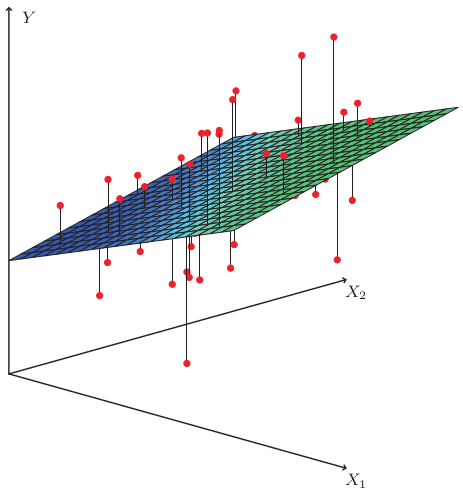
\includegraphics[width=.7\textwidth]{./chap/1chap/2sec/2images/1leastSquaresPlan.png}
  \caption{$n$ observations}
  \label{fig:2.1aLeastSquares}
\end{subfigure}%
\begin{subfigure}{.5\textwidth}
  \centering
	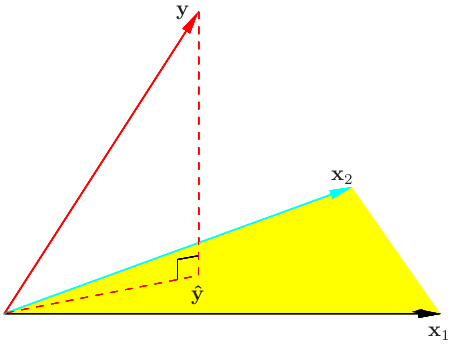
\includegraphics[width=\textwidth]{./chap/1chap/2sec/2images/11projection.png}
\caption{1 observation}
  \label{fig: 2.1bLeastSquares}
\end{subfigure}
  \caption{Least squares for a linear model with $2$ predictors of 
$p$-dimensions.}
\label{fig:test}
\end{figure}

\begin{align*}
\hat{\bm{y}} &=\bm{X}\hat{\beta}\\
	     &=\bm{X}\left(\bm{X}^{T}\bm{X}\right)^{-1}\bm{X}^{T}\bm{y}\\
	     &=\bm{H}\bm{y}
\end{align*}
$\bm{H}$ is called \tB{``hat'' matrix because it puts the hat on $\bm{y}$}.
\paragraph{Hat Matrix}
Residuals can also be expressed as a function of $\bm{H}$,
$\bm{\hat{e}} = \bm{y} - \bm{\hat{y}} = \bm{y} - \bm{Hy} = (\bm{I}-\bm{H})\bm{y}$.
It can be shown that \sB{$\bm{H}$ and $\bm{I}-\bm{H}$ are orthogonal projections}.\\
One can easily show that \tB{$\bm{H}\bm{H} = \bm{H}$} and $\left(\bm{I-H}\right)\left(\bm{I-H}\right)
= \bm{I-H}$

\subparagraph{Range and Kernel of the Hat Matrix}
$rank(\bm{X}) = rank(\bm{X}^{T}\bm{X}) = p^{*}$
\subparagraph{Residual and Fitted Values}
$\bm{H}(\bm{I}-\bm{H}) = \bm{H} -\bm{HH} = 0$, hence $\sP{\bm{\hat{y}}}{\bm{\hat{e}}} = 0$.
\tB{Therefore $\bm{\hat{y}}$ and $\bm{e}$ are orthogonal} in $\mathbb{R}^{n}$.
\subparagraph{Geometric interpretation}
The degrees of freedom associated with \tB{$\bm{\hat{y}}$ and $\bm{\hat{e}}$ can be seen to simply
be the dimensions of the respective vector subspace in which these 2 vectors have been projected}.\\
The vectors $\bm{y}, \bm{\hat{y}}$ and $\bm{\hat{e}}$ determine 3 points in $\mathbb{R}^{n}$ which
form a right-angled triangle, we can see the decomposition of total sum of squares into estimated
sum of squares and residual sum of squares as a special case of \emph{Pythagoras} theorem.
\subparagraph{Further information}
It might happen that the columns of \sB{$\bm{X}$ are not linearly independent, then
$\bm{X}^{T}\bm{X}$ is singular and the least squares coefficients $\hat{\beta}$ are not uniquely 
defined}.\\ 
Knowing that $\V{\bm{A}\bm{y}}=\bm{A}\V{\bm{y}}\bm{A}^{T}$:
\begin{center}
	\encB{$\V{\hat{\beta}}=\left(\bm{X}^{T}\bm{X}\right)^{-1}\sigma^{2}$}
\end{center}
a estimate of $\sigma^{2}$:$\hat{\sigma}^{2} = \dfrac{1}{N-p-1}\su{{i=1}}{N}(y_{i}-\hat{y}_{i})^{2}$ 
The $n-p-1$ rather than $n$ makes $\hat{\sigma}^{2}$ an unbiased
estimate.\\
$
\begin{cases}
\hat{\beta}\hookrightarrow\mathcal{N}\left(\beta, (\bm{X}^{T}\bm{X})^{-1}\sigma^{2}\right)\\
(n-p-1)\hat{\sigma}^{2}\hookrightarrow\sigma^{2}\chi_{n-p-1}^{2}
\end{cases}
$

\paragraph{Convexity}
Functions having a bowl shape with a unique minimum, more precisely:
$$\forall (\bm{\theta}, \bm{\theta'},\lambda) \in \mathcal{S}\times\mathcal{S}\times[0,1],
~ \lambda\bm{\theta} + (1-\lambda)\bm{\theta'} \in \mathcal{S} \Rightarrow \mathcal{S}
\text{ is \textbf{convex}}$$

%This is that we get after a linear regression.\\We recall that is we
%obtained for simple regressions:
%\begin{figure}[H]
%\centering
%\begin{minipage}{.5\textwidth}
%  \centering
%  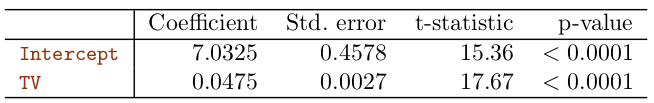
\includegraphics[width=\textwidth]{./chap/1chap/2sec/2images/2_1regressionTV.png}
%  \captionof{figure}{TV Regression}
%  \label{fig:test1}
%\end{minipage}%
%\begin{minipage}{.5\textwidth}
%  \centering
%  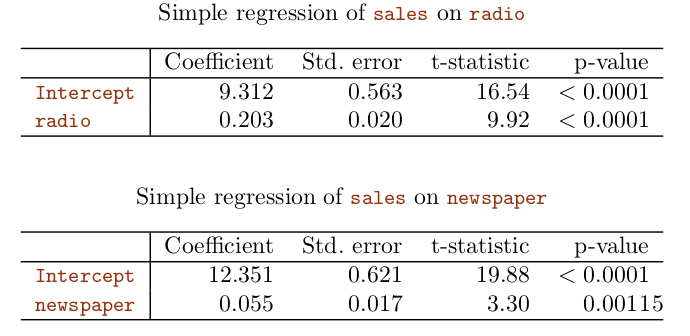
\includegraphics[width=\textwidth]{./chap/1chap/2sec/2images/2_2radioNewspapersRegression.png}
%  \captionof{figure}{NewspapersRegression}
%  \label{fig:test2}
%\end{minipage}
%\end{figure}
%For newspaper advertising we observe that results from simple 
%regression and those from multiple regression are opposites. Regarding
%correlation matrix markets where we spend more on radio we also tend to
%be spend more on newspaper advertising in those same markets.
%\begin{figure}[H]
%\centering
%\begin{minipage}{.5\textwidth}
%  \centering
%  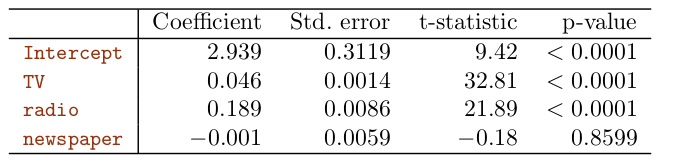
\includegraphics[width=\textwidth]{./chap/1chap/2sec/2images/2_3regressionMultiples.png}
%  \captionof{figure}{Regression multiples}
%  \label{fig:test1}
%\end{minipage}%
%\begin{minipage}{.5\textwidth}
%  \centering
%  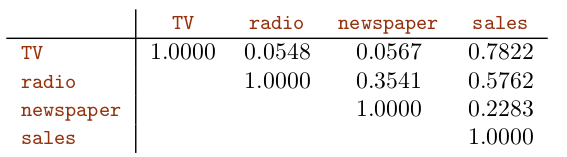
\includegraphics[width=\textwidth]{./chap/1chap/2sec/2images/2_4correlation.png}
%  \captionof{figure}{Correlation between predictors}
%  \label{fig:test2}
%\end{minipage}
%\end{figure}
\paragraph{Some important questions when we perform multiple linear
regression}
\begin{enumerate}
	\item Is at least one of the predictors $\left(X_{i}
		\right)_{1\leq i\leq p}$ useful in predicting the
		response?
	\item Do all the predictors help to explain $Y$ or is only a
		subset of the predictors useful?
	\item How well the model fit the data?
	\item Given a set of predictor values, what response values
		should we predict, and how accurate is our prediction?
\end{enumerate}
\subparagraph{Is there a relationship between the predictors and the
responses?}
$\begin{cases}
	H_{0}:\forall i\in\inter{1}{p} \beta_{i}=0\\
	H_{a}:\exists j\in\inter{1}{p} \beta_{j}\neq 0
\end{cases}$\\This hypothesis test is performed by computing the \emph{
F-statistic}:
\begin{center}
	\encN{$F=\dfrac{\frac{TSS-RSS}{p}}{\frac{RSS}{n-p-1}}$}
\end{center}
If the linear model assumptions are correct, one can show that:\\
$\begin{cases}
	\E{\dfrac{RSS}{n-p-1}}=\sigma^{2}\\
	\E{\dfrac{TSS-RSS}{p}}=\sigma^{2}\text{ and that provided }
	H_{0}\text{ is true.}
\end{cases}$\\Then \tB{when there is no relationship between 
predictors and the response, on would expect the \emph{F-statistic} to
take on a value close to $1$}. If $H_{a}$ is true, $\E{\dfrac{TSS-RSS}{
p}}>\sigma^{2}$, so we expect F greater than $1$.
%\begin{figure}[H]
%	\begin{center}
%		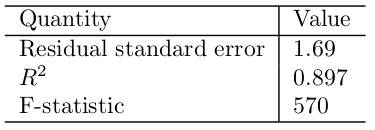
\includegraphics[width=.5\textwidth]{./chap/1chap/2sec/2images/2_5Fstatistic.png}
%	\end{center}
%	\caption{F-statistic for the multiple regression model obtained
%	by regressing sales onto radio, TV and newspaper.}
%	\label{fig:1}
%\end{figure}
Since this is far larger than 1, it provides compelling evidences
against $H_{0}$.\\When $n$ is large an F-statistic that is just little
larger than $1$ might still provide evidence against $H_{0}$. In 
contrast when $n$ is small a larger \emph{F-statistic} is needed to
reject $H_{0}$.\Moi{Any statistical software can be used to compute
the \emph{$p$-value} associated with the \emph{F-statistic}, based on
this \emph{$p$-value} we can determine whether or not reject $H_{0}$}\\
Sometimes we need to test that a particular subset of $q$ of the $p$
coefficients are zero, then:\\$H_{0}:\forall i\in\inter{1}{n} 
\beta_{p-q+i}$ in this case we fit a second model that uses all 
variables except those last $q$. Suppose that the residual sum of 
squares for that model is $RSS_{0}$ then:\\$F=\dfrac{\frac{RSS_{0}-RSS}
{q}}{\frac{RSS}{n-p-1}}$.\\If we use \emph{$p$-values} associated to the
$t-statistic$ we might find a non-null percentage of small \emph{
$p$-values}, and then wrongly to think that there is relationship
between a few predictors and the response.\\Hence we always must to use
\emph{\tR{$p$-values associated with F-statistic}} in multiple regression
case.\\The \emph{F-statistic} approach works well when \emph{\tV{$p$ is
relatively small, and certainly small compared to $n$}}, if not the
case we \tR{cannot use F-statistic approach} see to chapter $6$.\\

\tR{For a multiple regression}
To test the hypothesis that a particular coefficient $\beta_{j}=0$, we
form the standardized coefficient or $Z$-score:
\begin{center}
	$z_{j}=\dfrac{\hat{\beta}_{j}}{\hat{\sigma}\sqrt{\nu_{j}}}$
\end{center}
$\nu_{j}$ is the $j^{th}$ diagonal element of $\left(X^{T}X\right)^{-1}$
$H_{0}: \beta_{j}=0$, $z_{j}$ is distributed as $t_{N-p-1}$ and hence
a large absolute value of $z_{j}$ will lead to rejection of this 
null hypothesis.\\
Often we need to test the significance of groups of coefficients 
simultaneously, here we use the $F$-statistic.
\begin{center}
	$F=\dfrac{\frac{RSS_{0}-RSS_{1}}{p_{1}-p_{0}}}{\frac{RSS_{1}}{N-p_{1}-1}}$
\end{center}
$RSS_{1}$ is the residual sum of squares for the least squares fit of 
the bigger model with $p_{1}+1$ parameters, and $RSS_{0}$ the same for
the nested smaller model with $p_{0}+1$ parameters, having $p_{1}-
p_{0}$ parameters constrained to be zero.\\
The $F$-statistic measures the change in residual sum-of-squares per 
additional parameters in the bigger model.\\
Under the Gaussian assumptions and the null hypothesis that the smaller
model is correct the $F$ statistic will have a $F_{p_{1}-p_{0},N-p_{1}-1}$ distribution.\\
We can isolate $\beta_{j}$ to obtain a $1-2\alpha$ confidence interval
for $\beta_{j}$:
\begin{center}
	$\left(\hat{\beta}_{j}-z^{1-\alpha}\sqrt{\nu_{j}}\hat{\sigma}, \hat{\beta}_{j}-z^{1-\alpha}\sqrt{\nu_{j}}\hat{\sigma}\right)$
\end{center}
\paragraph{The Gauss-Markov Theorem}
$\hat{\theta}=c^{T}y$ an unbiased estimate for $a^{T}\beta$,
$\E{c^{T}y}=a^{T}\beta\Rightarrow \V{a^{T}\hat{\beta}}\leq\V{c^{T}y}$\\
The Gauss-Markov theorem implies that \tB{the least squares estimator has 
the smallest mean squared error of all linear estimators with no bias}.

\paragraph{Regression by Successive Orthogonalisation (Gram-Schmidt)}
\tR{Only applicable on linearly independents matrix/vector family}
\subparagraph{Algorithm}
\begin{figure}[H]
	\begin{center}
		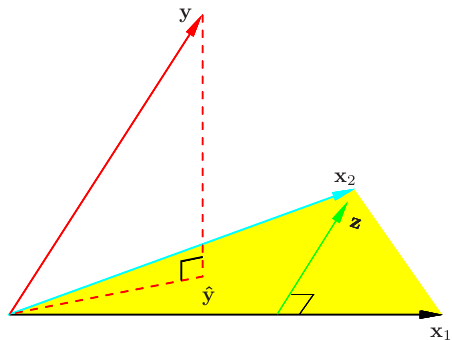
\includegraphics[width=.5\textwidth]{./chap/1chap/2sec/2images/3_1regressionImage.png}
	\end{center}
	\caption{The vector $\bm{x}_{2}$ is regressed on the vector
	$\bm{x}_{1}$, leaving the residual vector $\bm{z}$. The 
	regression of $\bm{y}$ on $\bm{z}$ gives the multiple 
	regression coefficient of $\bm{x}_{2}$.\\
	Adding together the projections of $\bm{y}$ on each of 
	$\bm{x}_{1}$ and $\bm{z}$ gives the least squares fit 
	$\hat{\bm{y}}$}
	\label{fig:3.1regressionImage}
\end{figure}
\begin{enumerate}
	\item Initialize $\bm{z}_{0}=\bm{x}_{0}=\bm{1}$
	\item $\forall j\in\inter{1}{p}$:
		Regress to $\bm{x}_{j}$ on $\prtH{\bm{z}}{j}{0}{j-1}$
		to produce:
		\begin{itemize}
			\item coefficients for $k\in\inter{0}{j-1}
				\hat{\gamma}_{kj}=
				\dfrac{<z_{l}|x_{j}>}{<z_{l}|z_{l}>}$
			\item residual vector $z_{j}= x_{j}-\su{{k=0}}{j-1}\hat{\gamma}_{kj}z_{k}$
		\end{itemize} 
	\item Regress $\bm{y}$ on the residual $\bm{z}_{p}$ to give the
		estimate $\hat{\beta}_{p}$
\end{enumerate}
\begin{center}
$\bm{X} = \bm{Z}\bm{\Gamma}$
\end{center}
$\bm{Z}$ has as column the $z_{j}$ (orthogonalised $x_{j}$), 
$\bm{\Gamma}$ is the upper triangular matrix with entries 
$\hat{\gamma}_{kj}=\dfrac{<z_{k}|x_{j}>}{<z_{k}|z_{k}>}$\\
Introducing the diagonal matrix $\bm{D}$ such as $\bm{D}_{jj} = 
\norm{\bm{z}_{j}}$ we get: 
\begin{align*}
	\bm{X} &= \bm{Z}\bm{D}^{-1}\bm{D}\bm{\Gamma}\\
	&= \bm{Q}\bm{R}
\end{align*}
the so-called $QR$ decomposition of $\bm{X}$. Here $\bm{Q}$ is an 
orthogonal matrix $\bm{Q}^{T}\bm{Q}=\bm{I}$ and $\bm{R}$ is a 
$(p+1)\times(p+1)$ upper triangular matrix\\
Then: \\
$
\begin{cases}
	\hat{\beta} = \bm{R}^{-1}\bm{Q}^{T}\bm{y}\\
	\hat{\bm{y}}= \bm{Q}\bm{Q}^{T}\bm{y}
\end{cases}
$
\subparagraph{Python code}:
\begin{python}
import numpy as np
X = np.random.randn(9, 6)
Q, R = np.linalg.qr(X)
beta_coef = (np.linal.inv(R).dot(Q.transpose()
    )).dot(y)
y_hat = (Q.dot(Q.transpose())).dot(y)
\end{python}

\subparagraph{R code}:
\begin{rcode}[deletekeywords={beta, coef, hat}]
X <- replicate(6,rnorm(9))
qq <- qr.Q(X)
rr <- qr.R(X)
beta.coef <- matrix.inverse(rr)%*%transpose(qq)%*%y
y.hat <- qq%*%transpose(qq)%*%y
\end{rcode}

\paragraph{Multiple Outputs}
\begin{align*}
	Y_{k} &= \beta_{0k} + \su{{j=1}}{p}X_{j}\beta_{jk}+\epsilon_{k}\\
&= f_{k}(\bm{X})+\epsilon_{k}
\end{align*}
In matrix notation: $\bm{Y}=\bm{X}\bm{B} + \bm{E}$\\
$\bm{Y}$ is the $N\times K$ response matrix, $\bm{X}$ is the 
$N\times(p+1)$ input matrix, $\bm{B}$ is the $(p+1)\times K$ matrix of
parameters and $\bm{E}$ is the $N\times K$ matrix of errors.\\
\begin{align*}
	RSS(\bm{B}) &= \su{{k=1}}{K}\su{{i=1}}{N}\left(y_{ik}-f_{k}(x_{i})\right)^{2}\\
	&= tr\left[ (\bm{Y}-\bm{XB})^{T}(\bm{Y}-\bm{XB}) \right]
\end{align*}
$\hat{\bm{B}}=(\bm{X}^{T}\bm{X})^{-1}\bm{X}^{T}\bm{Y}$
If the errors $\epsilon=\prth{\epsilon}{i}{K}$ are correlated :
$RSS(\bm{B}; \bm{\Sigma})=\su{{i=1}}(y_{i}-f(x_{i}))^{T}\Sigma^{-1}(y_{i}-f(x_{i}))$
with $\Sigma^{-1}=Cov(\epsilon)$


%\subparagraph{Deciding on important variables}
%Ideally we would like to perform variable selection by trying out a lot
%of different models, each containing a different subset of predictors.
%But there are $2^{p}$ models that contains subsets of $p$ predictors.\\
%Then we use $3$ classical approaches for this selection:
%\begin{enumerate}
%	\item \emph{\tB{Forward selection}}:
%		\begin{itemize}
%			\item We begin with a \sB{model containing 
%				intercept but no predictors}.
%			\item Fit $p$ simple regressions \& add to the
%				null model the variable with that 
%				results in the lowest RSS
%			\item Add to that model the that results in the
%				lowest RSS for the new $2$-variable
%				model.
%			item To continue this approach until some
%				stopping rule is satisfied
%			\item
%Python code:
%\begin{python}
%import sklearn
%from sklearn import linear_model
%import mlxtend
%from mlxtend.feature_selection import SequentialFeatureSelector as SFS
%
%df = pd.read_csv(`myfile.csv`, sep=`;`)
%X = df.iloc[:,1:] 
%y = df.iloc[:,:1]
%reg = linear_model.LinearRegression()
%sfs1 = SFS(reg,
%    k_feature = np.arange(X.shape[1]) # number of features to select
%    forward = True,         # backward selection otherwise
%    floating=False,         # adds a conditional exclusion/inclusion if True
%    verbose = 2,            # Level of verbosity to use in logging (0 to 2)
%    scoring=`accuracy`,     # if None, uses `accuracy` for sklearn classifiers and `r2` for sklearn regressiors
%    cv=5                    # for k-fold cross-validation
%)
%sfs1_model = sfs1.fit(X, y)
%sfs1.subsets_
%\end{python}
%		\end{itemize}
%	\item \emph{\tB{Backward selection}}:
%		\begin{itemize}
%			\item Start with all variables in the model \&
%				remove the variable with the largest
%				\emph{p-value} (the variable the least
%				statistically significant).
%			\item Fit the new $p-1$-variable model and
%				remove the variable with the largest
%				\emph{p-value}.
%				
%			\item Continue untill a stopping rule is 
%				reached (for example we may stop when
%				all remaining variables have a \emph{
%				p-value} below some threshold).
%		\end{itemize}
%	\item \emph{\tV{Mixed selection}}
%		\begin{itemize}
%			\item Start with \sV{no variables in the model}
%			\item As with \emph{forward selection} add the
%				variable that provides the best fit
%			\item The \emph{p-value} of variables can 
%				become larger as new predictors are
%				added to the model. Hence if at any 
%				point the \emph{p-value} for one of the
%				variables in the model rises above a
%				certain threshold, then we remove that
%				variable from the model
%			\item Continue to perform these forward and
%				backward steps untill all variable in
%				the model have a sufficiently low 
%				\emph{p-value}, and all variable 
%				outside would have a large \emph{
%				p-value} if added to the model.
%			\item Take the previous code and edit the line associated with floating:
%\begin{lstlisting}
%floating = True
%\end{lstlisting}
%		\end{itemize}
%\end{enumerate}
%\emph{Backward selection} \sR{cannot be used when $p>n$}\\
%\emph{Forward selection} is a \sO{very greedy approach}, and might
%include variables early that later become redundant.\\
%\tV{\emph{Mixed selection} can remedy this}.
\subparagraph{Model fit}
Recall that in \sB{simple regression $R^{2}=Cor\left(X,Y\right)^{2}$}
the square of the correlation between predictor and the response. Where
as in multiple multiple regression \sR{$R^{2}=Cor\left(\widehat{Y},Y
\right)^{2}$}, in fact one property of the fitted model is it maximizes
this correlation among all possible linear model.\\ \tB{$R^{2}$ will
always increase when more variables are added even though those
variables are weakly associated with the response}.\Moi{this due to the
fact that adding another variable to least square equations to fit the
training data more accurately}.
\begin{center}
	\enc{$RSE=\sqrt{\dfrac{1}{n-p-1}RSS}$}
\end{center}
\sN{In addition to looking RSE and $R^{2}$ it can be useful to plot the
data}.
\begin{figure}[H]
	\begin{center}
		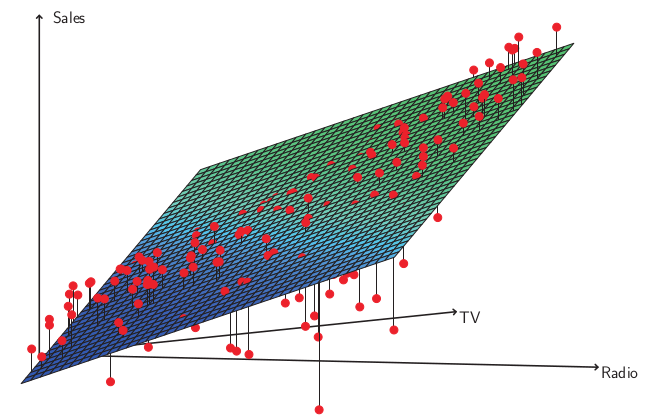
\includegraphics[width=\textwidth]{./chap/1chap/2sec/2images/2_6dataPlot.png}
	\end{center}
	\caption{We can see that there is a pronounced non-linear
	relationship in data.\\Positive residuals  tend to lie along
	the 45-degree line, the negative residuals tend to lie away 
	from this line where budgets are more lopsided.}
	\label{fig:fig 2.6}
\end{figure}
It suggests \tR{synergy} between advertising media, whereby combining
media together results in a bigger boost to sales than using any single
media.
\subparagraph{Prediction}
Even though after the multiple regression model fitting it is
straightforward to compute linear combination in order to get 
$\widehat{Y}$ there are \sO{3 sorts of uncertainty associated with this
prediction}:
\begin{enumerate}
	\item The \tO{inaccuracy in $\prth{\widehat{\beta_{i}}}{i}{n}$}
		which is related to the \sN{reductible error}
	\item The \tO{model bias} which results in the fact that our
		models are approximations of the reality.
	\item The \tO{irreducible error}
\end{enumerate}
